\documentclass[10pt]{article}
\usepackage[utf8]{inputenc}
\usepackage{amsmath}
\usepackage{amsfonts}
\usepackage{tikz}
\usepackage{amssymb}
%\usepackage{fullpage}
\usepackage[top=1in, bottom=1in, left=1in, right=1in]{geometry}
\usepackage{graphicx}
\usepackage{hyperref}
\usepackage{subcaption}
\usepackage{float}
\usepackage[section]{placeins}
\graphicspath{{./FigJar/}}
\begin{document}
\author{Erdem M. Karaköylü}
\title{A Bayesian Approach to OC4}
\date{\today}
\maketitle
\tableofcontents
\newpage

\newcommand{\reddash}{\raisebox{2pt}{\tikz{\draw[-,red,dashed,line width=1.2pt](0,0) -- (5mm,0);}}}
\newcommand{\blkdash}{\raisebox{2pt}{\tikz{\draw[-,black,dashed,line width=1.2pt](0,0) -- (5mm,0);}}}
\newcommand{\blksold}{\raisebox{2pt}{\tikz{\draw[-,black,solid,line width=1.2pt](0,0) -- (5mm,0);}}}

\section{Background}

A number of approaches have been proposed to derive chlorophyll concentration from remote sensing reflectance (\textit{Rrs}). The two main paradigms are semi-analytical and empirical. Semi-analytical approaches are more easily interpretable as they are built at least in part on a mechanistic understanding of the processes at play. The highly variable nature of satellite oceanography in general, and ocean color in particular, has made this approach challenging in that so far a consistently satisfactory performance remains elusive. The 
The Regression Model:
\begin{align}
log_{10}\left(chlor_a\right) = a_0 + \sum_{i=1}^ja_ilog_{10}\left(\frac{max\left(Rrs\left(\lambda_{blue}\right)\right)}{Rrs\left(\lambda_{green}\right)}\right)
\end{align}


\section{Issues with ordinary least squares (ols)}
There are a number of shortcomings that makes \textit{ols} unsuitable for developing the model above. I'll briefly outline some shortcomings of OLS; first, general issues with \textit{ols}, then issues specific to the development of $OC_4$
	\subsection{General shortcomings}
	\begin{itemize}
		\item $R^2$ as a diagnostic encourages a higher number of parameters
		\item Almost garanteed to overfit on the training data.
	\end{itemize}
	
	\subsection{Specific shortcomings}
	\begin{itemize}
		\item polynomial regression inherently affected by multicollinearity
		\item lack of testing simpler formulations
		\item data paucity
	\end{itemize}
		
\section{Bayesian paradigm}
	\subsection{Pros and cons of being a bayesian}
		\subsubsection{a perception problem}
		\subsubsection{uncertainty}
		\subsubsection{on the use of priors}		
	\subsection{Bayes'rule}
	Bayes' rule is relatively straightforward. Given two events A and B that are not independent,
	their joint probability $P(A,B)$ can be written in two different ways:
	\begin{align}
		P(A,B) = P(A|B) \times P(B) = P(B|A)\times P(A)	
	\end{align}
	
	

	The above becomes quite handy when one of the conditional probabilities, say $P(B|A)$ is harder to compute than the other. This is easily dealt with by rearraging the terms above, which leads to Baye's rule:
	\begin{align}
		P(B|A)  = \frac{P(A|B) \times P(B)}{P(A)}
	\end{align}
	
	In the context of scientific enquiry, conditional probabilities allow relating hypotheses to collected data, by way of model formulation. Given a set of hypotheses, $H$, that address a specific question, and given a data set, $D$, collected to estimate the validity of these hypotheses, (3) can be rewritten as:
	\begin{align}
		P(H|D) = \frac{P(D|H) \times P(H)}{P(D)}
	\end{align}
	A bit of vocabulary is in order here:
	\begin{itemize}
		\item $P(H)$: \textbf{the prior} - This is the belief of the experimenter \textit{prior} to seeing the data. 
		\item $P(D|H)$: \textbf{the likelihood} - While frequentists will tell you that this is what you want and that you should maximize it to approach the "truth", that is seldom correct and a great way to overfit the model to the training data, thereby leading to poor prediction of unseen data. More about this later.
		\item $P(D)$: \textbf{the evidence} - For the purpose of this paper, it's enough to refer to it as a normalizing constant that basically makes sure that the probabilities computed through (4) sum to 1. One of the main tools of bayesian inference, and one that I will use further below, the Markov Chain Monte Carlo (MCMC) sampler does away with this otherwise often computatiationally intractable construct.
		\item $P(H|D)$: \textbf{the posterior} - This is the set of probabilities that allow to enable the most likely hypotheses, and provides in the process uncertainties around the chose estimates.
	\end{itemize}
	\subsection{Warm-up: Inferring Earth's Land proportion}
		I stole and modified this example from McElreath (2015). The goal here is to infer the proportion of land. The hypotheses are then all the possible values that this proportion parameter, ranging from 0 to 1. The steps are as follows:
		\subsubsection{defining a prior}
			\begin{itemize}
				\item $P(H)$
				\item can be vague or specific, depending on the researcher's prior knowledge
				\item prior formulation is akin to placing bets on a roulette table
				\item a vague prior will rapidly get overwhelmed by the collected data
				\item a vague prior may lead to overfitting
				\item a strong (regularizing) prior will "calm" the model - a large dataset will overwhelm it				
				\item a strong prior may lead to underfitting
			\end{itemize}
		\FloatBarrier
		\subsubsection{collect data}
			%\FloatBarrier
			\begin{itemize}
				\item random sampling of locations (Fig. 1)
				\item land? water?
				\item define the likelihood model (more about this later)
				\item compute likelihood of data given hypotheses; $P(D|H)$
			\end{itemize}					
			\begin{figure}[H]
				\centering
				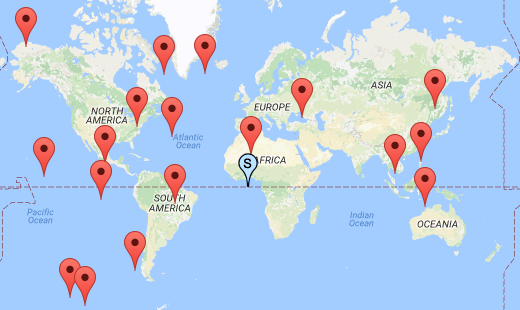
\includegraphics[scale=0.5]{randomMapPts.png}
				\caption{Random sampling of 18 geographic locations}
			\end{figure}
		\FloatBarrier
		\subsubsection{update hypotheses probability given new data}
%			$P(D|H)\times P(H)$
			\begin{figure}[H]
				\centering
				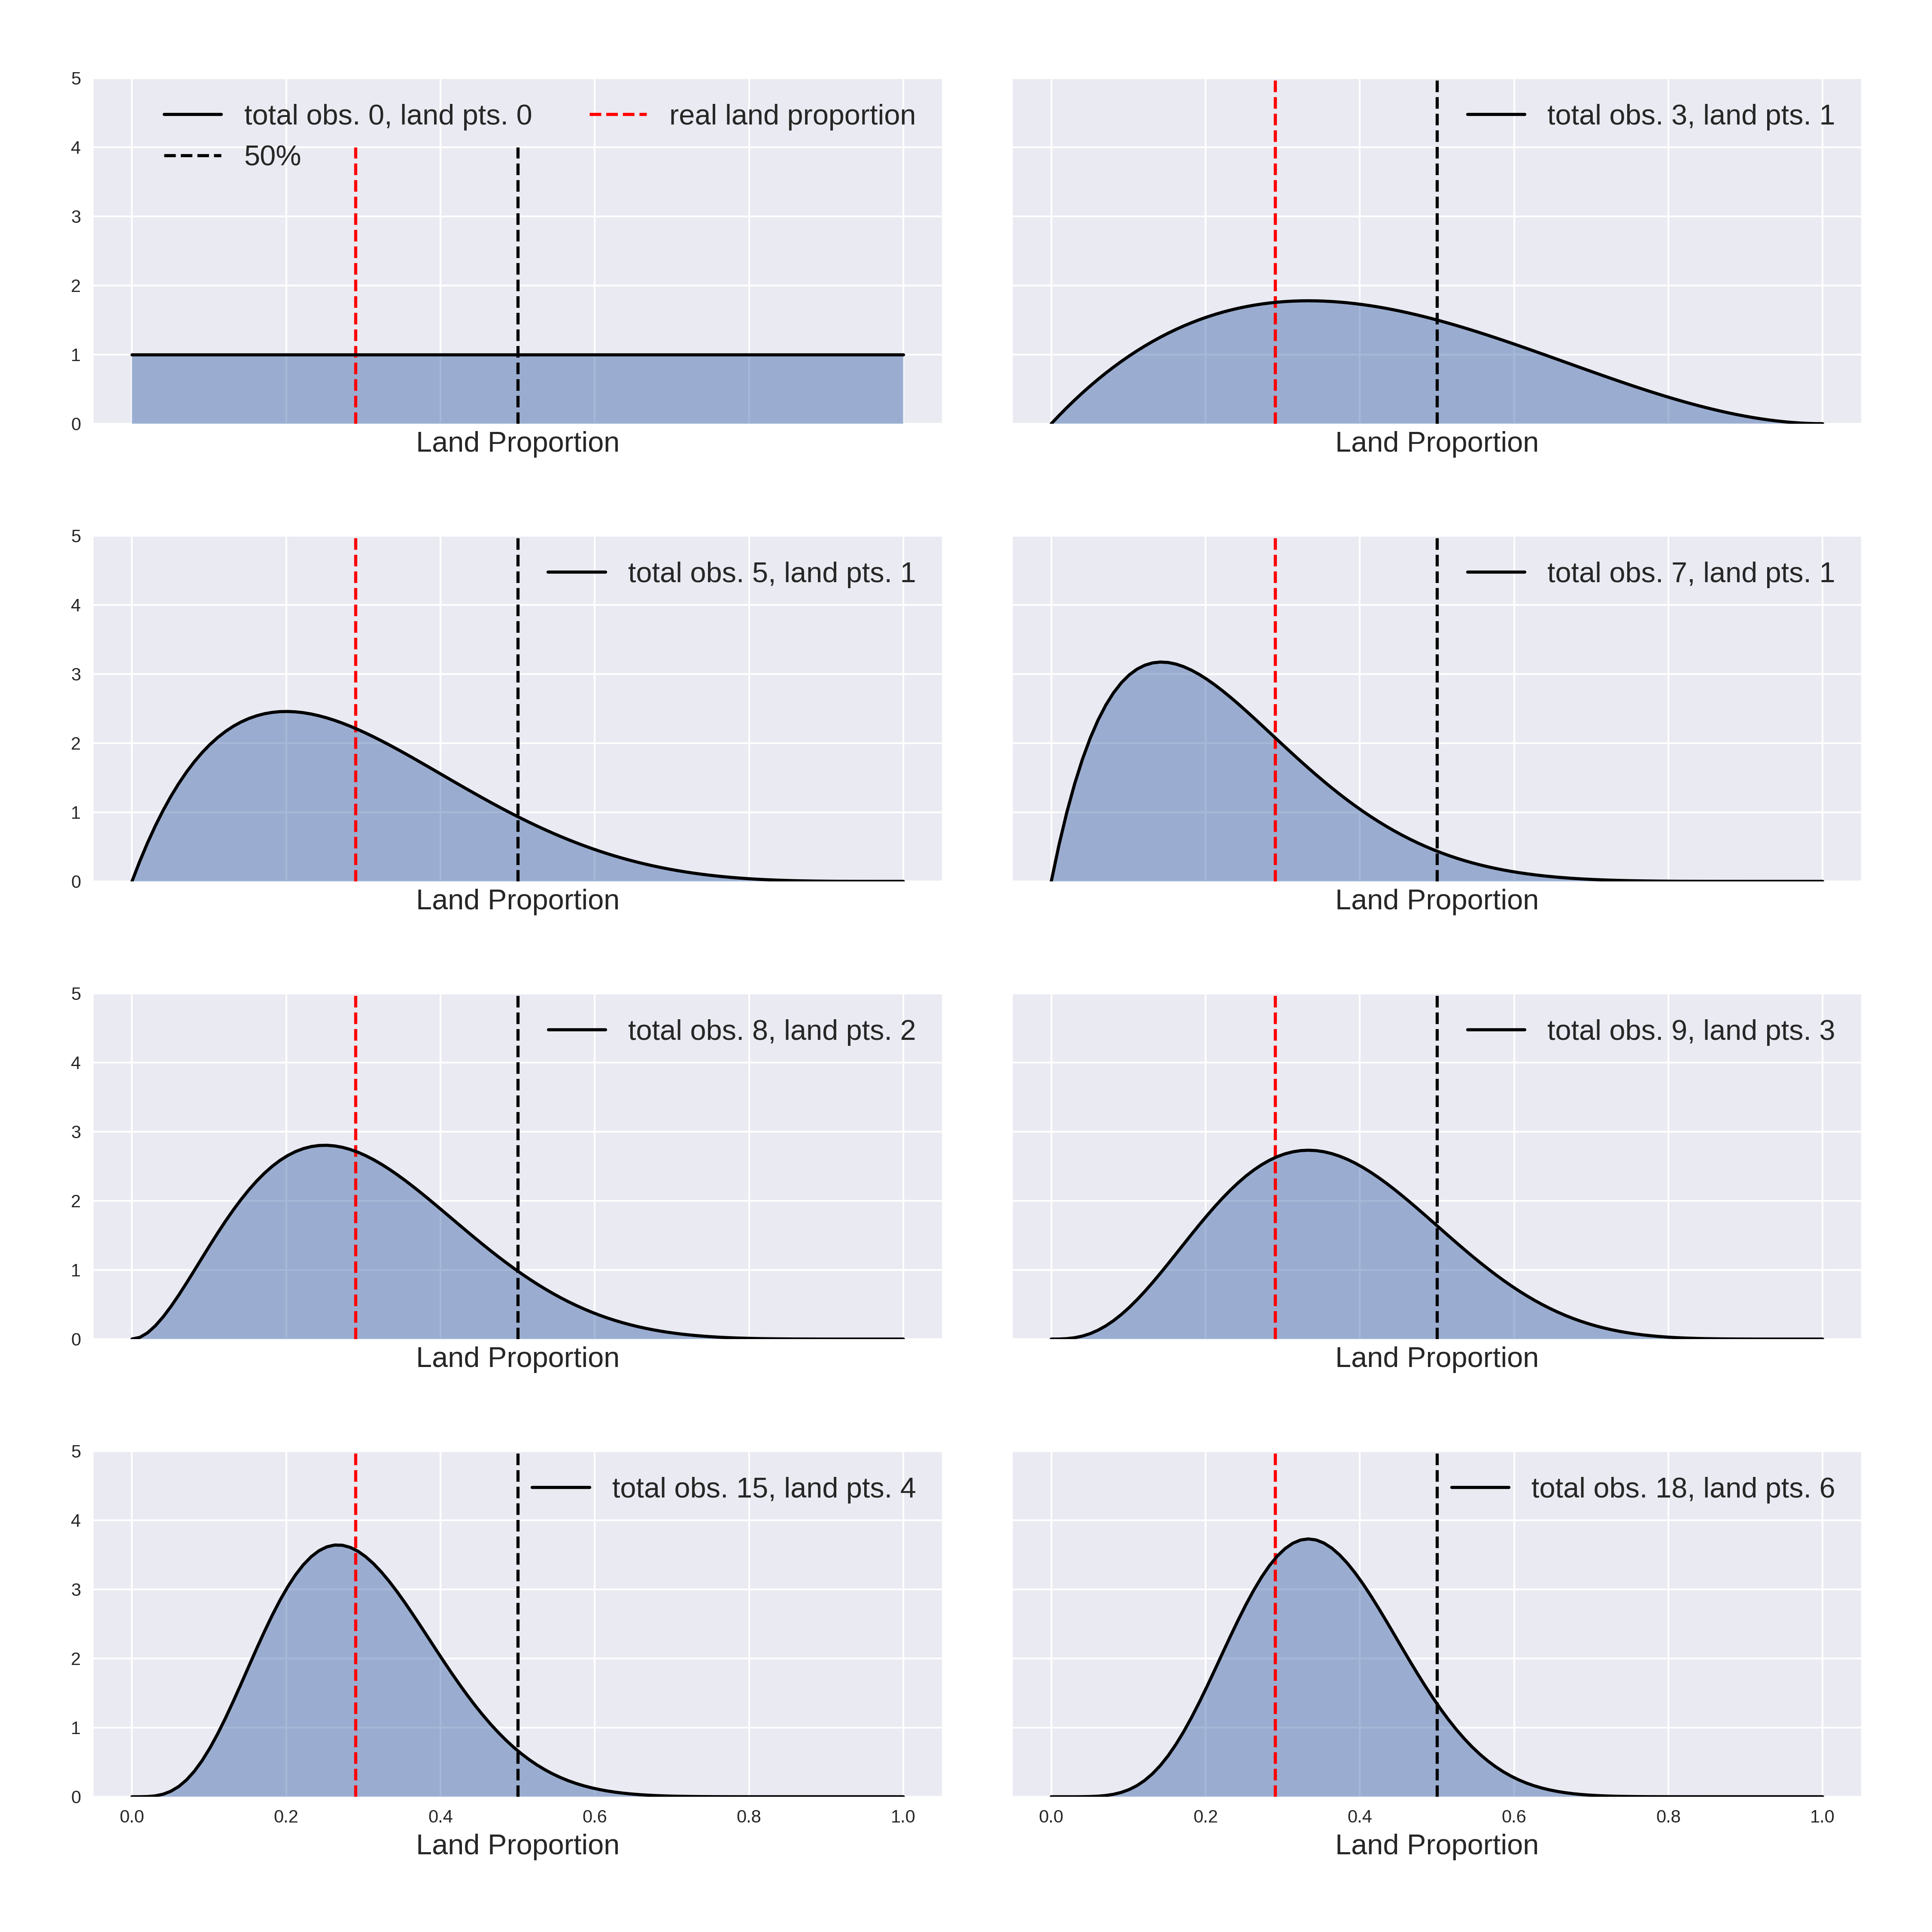
\includegraphics[scale=0.35]{landProp_flat.png}
				\caption{Inference starting from a flat uniform prior (top left panel). The inference progresses top-down and left-right.
				\protect\reddash: true proportion sought;
				\protect\blkdash: 50 land/water reference;
				\protect\blksold: distribution inferred from combining data-driven likelihood with prior.}
			\end{figure}%
			\begin{figure}[H]
				\centering
				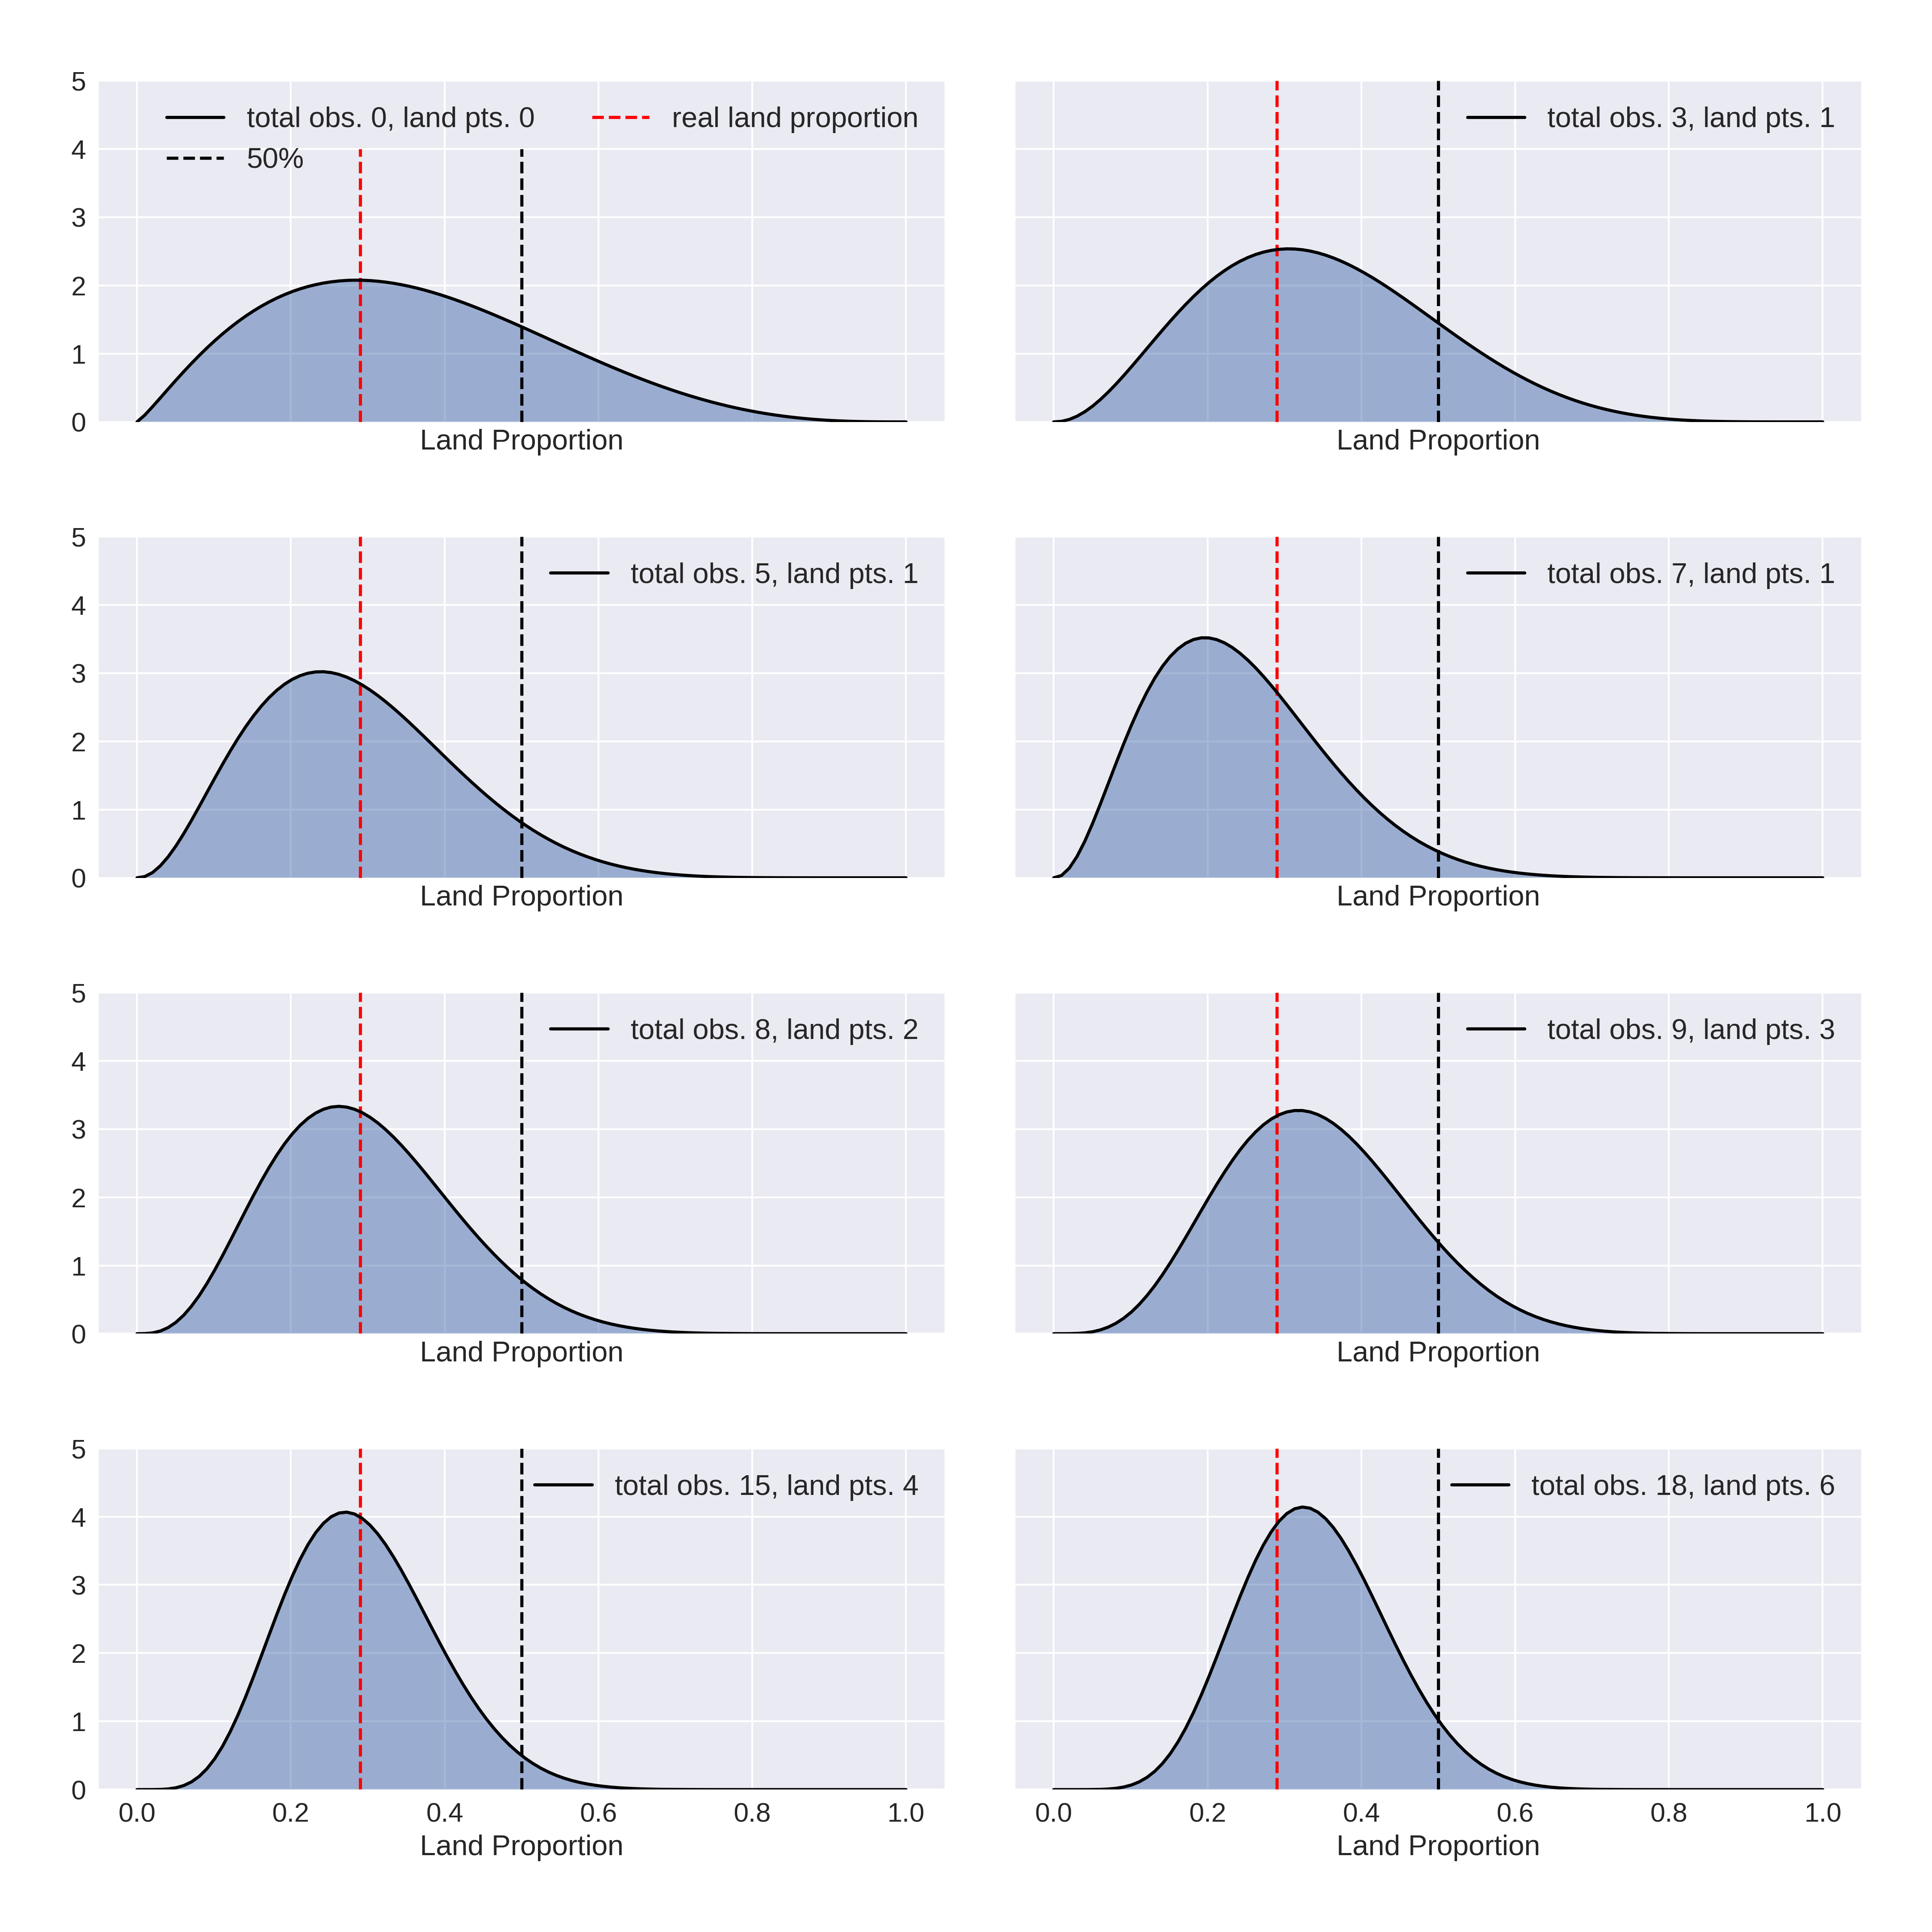
\includegraphics[scale=0.35]{landProp_weak.png}
				\caption{Starting from a weak beta prior}
			\end{figure}%
\section{Bayesian development of OC4}
	\subsection{Data overview}
		\begin{figure}[H]
				\centering
				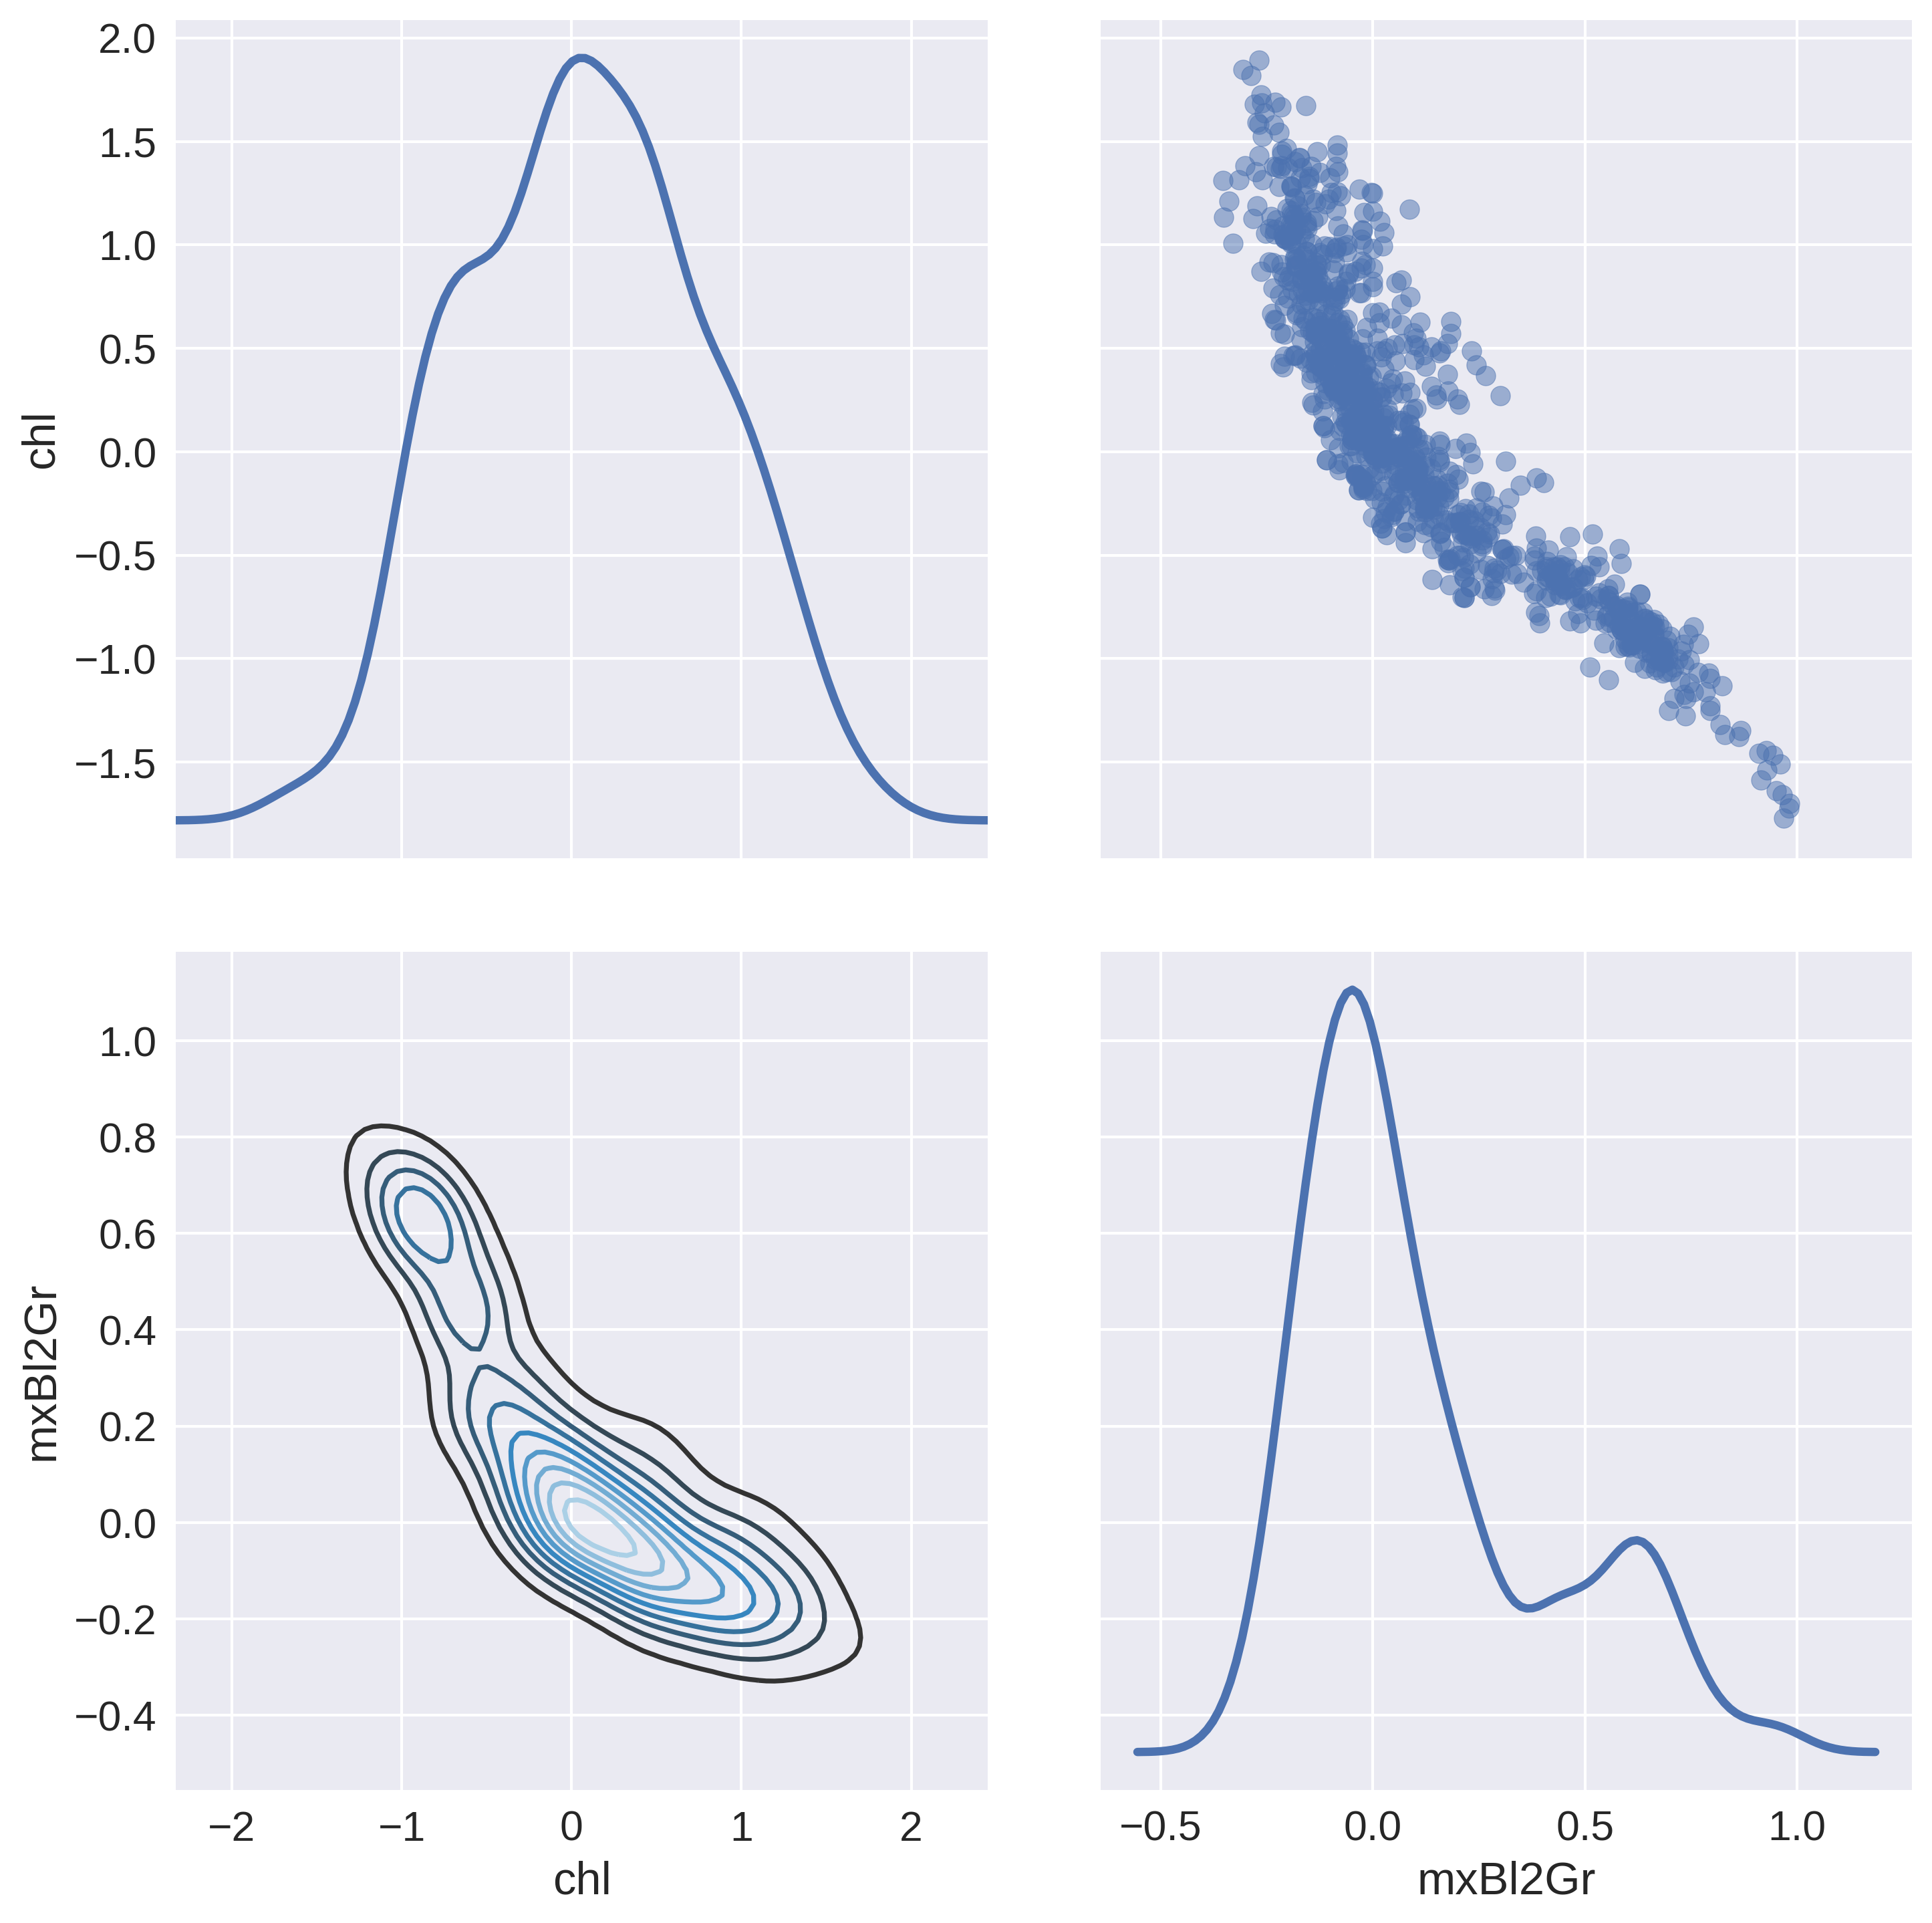
\includegraphics[scale=0.4]{dataOverview.png}
				\caption{NOMAD data used for model development.\\chl: $log_{10}(chl_{\textit{a}})$;
						 mxBl2Gr: $log_{10}\frac{max(Rrs_{443, 490, 510})}{Rrs_{555}}$}
			\end{figure}%
	\subsection{Models and priors}
	\subsection{Fitting and Diagnostics}
	
\newpage
\section{Bayesian Model Evaluation}
	\subsection{Posterior predictive checks (\textit{PPC})}
	\subsubsection{in-sample}
	\subsubsection{out-of-sample}
	\subsection{Information criteria and model evaluations}
	
\newpage
\section{Developing Alternative Empirical Models}
	\subsection{Linear Models}
	\subsection{Hierarchical Models}
	\subsection{Partially Pooled Models}
	\subsection{Bayesian Neural Networks}
\end{document}